\documentclass{beamer}
\usepackage{listings}
\usetheme{Copenhagen}
\usecolortheme{beaver}
\setbeamertemplate{navigation symbols}{}
\setbeamertemplate{footline}{\parbox[t][12pt][c]{12pt}{~\scriptsize\insertframenumber}}
% \usepackage{beamerthemesplit} // Activate for custom appearance

%%%%%%%%%%%%
% MVS: Language definitions
%
\renewcommand{\ttdefault}{pcr}
\lstset{
  basicstyle=\small\ttfamily,
  breaklines=true
}
\lstdefinelanguage{cvl}{
  morekeywords={generalize,to, with, other, at, zoom, levels, weigh, by, subject, and, create, constraint, as, not, exists, resolve, if, delete, select, from, where, in, order, over, setup, teardown,force,min,level,for,allornothing,join,on,setup,group,having,index,temporary,table,drop,partition,merge,partitions},
  sensitive=false,
  morecomment=[l]{//},
  morecomment=[s]{/*}{*/},
  morestring=[b]",
}
\lstset{
  language=cvl
}


\title{Declarative Cartography}
\subtitle{In-Database Map Generalization of Spatial Datasets}
\author{\underline{Pimin Konstantin Kefaloukos}, Marcos Vaz Salles, \\Martin Zachariasen\\ \small{\emph{Computer Science Department (DIKU)}, \textbf{University of Copenhagen}}}
\date{\today}

\begin{document}

\frame{\titlepage}

\frame
{
  \frametitle{Motivation}
  \begin{itemize}
  \item \textbf{Imagine}: you're a \emph{journalist} and want to tell a story about restaurants in Z\"{u}rich \emph{using a map}.
  \item \textbf{Database}: You have a \emph{database} of restaurants (unique ID, location, star rating, name etc.)
  \item Simply showing all the records creates a mess (see picture)
  \item \textbf{Generalization}: It would be nice if the database could generalize the data for you!
  \end{itemize}
  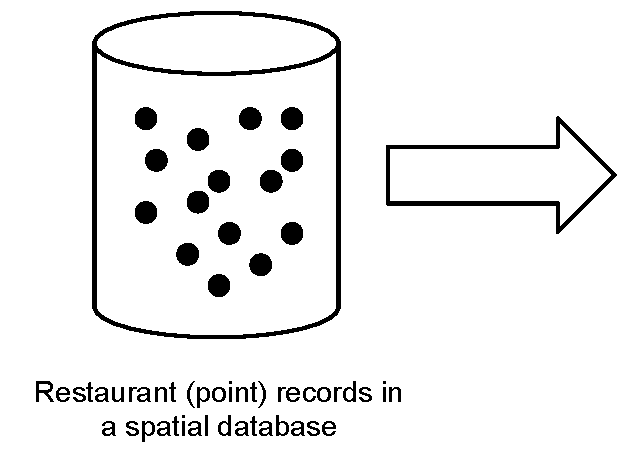
\includegraphics[scale=0.5]{figs/spatial-database-with-points.pdf} 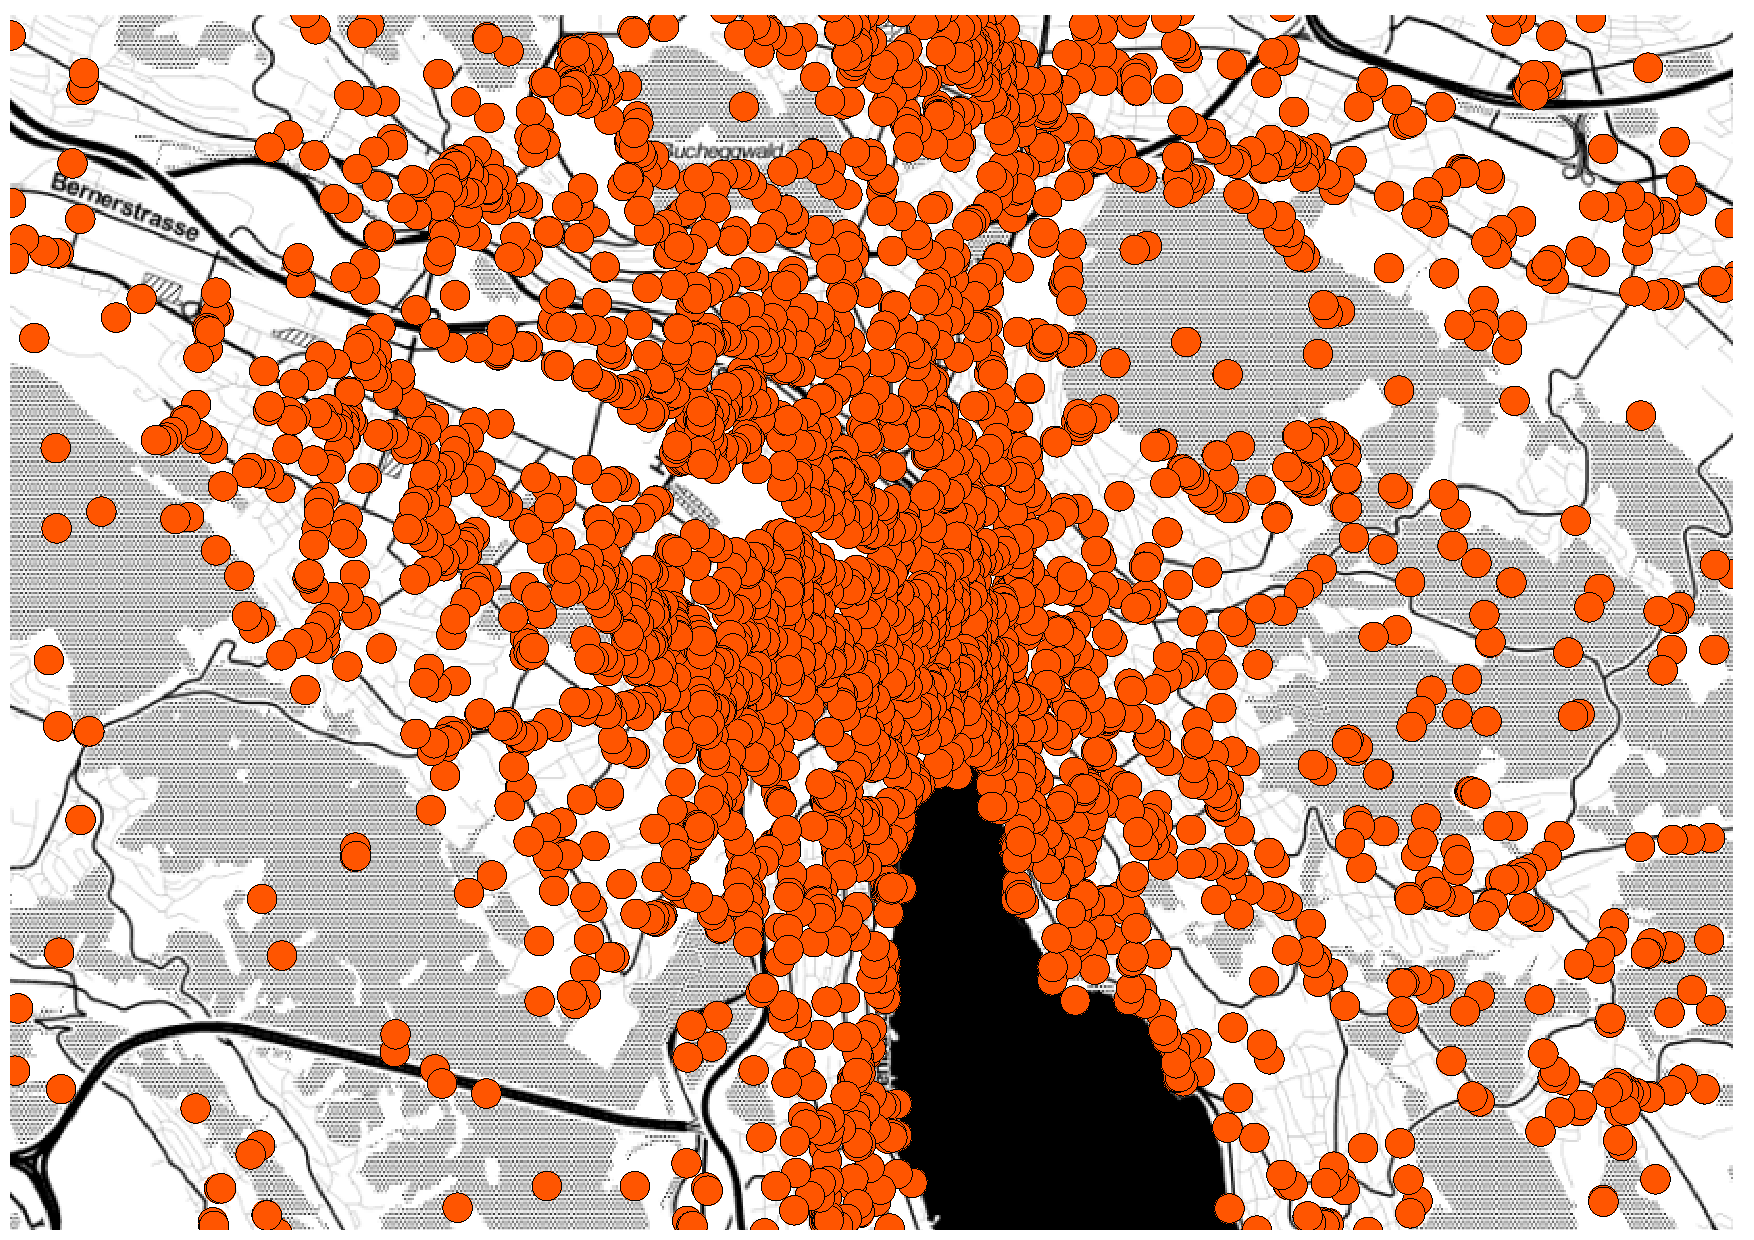
\includegraphics[scale=0.18]{figs/zurich-unfiltered.pdf}
}

% Setting stage
\frame[t]
{
  \frametitle{What a good (thematic) map might look like}
\begin{columns}[t]
	\begin{column}[l]{6cm}
		\begin{itemize}[<+->]
			\item Records should appear \emph{gradually} when zooming in, i.e. \emph{constant information~density}
			\item ``Important'' records should get priority
			\item Visible records should \emph{remain visible} when zooming in
			\item There should be some way of controlling \emph{layout}
			\item It would be nice if you get state all these things in an \underline{easy way}
		\end{itemize}
	\end{column}
	\begin{column}[l]{6cm}
    \begin{figure}
        \includegraphics<1>[scale=0.18]{figs/zoom12.pdf}
        \includegraphics<2>[scale=0.18]{figs/zoom13.pdf}
        \includegraphics<3>[scale=0.18]{figs/zoom14.pdf}
        \includegraphics<4>[scale=0.18]{figs/zoom15.pdf}
        \includegraphics<5>[scale=0.18]{figs/zoom16.pdf}
    \end{figure}                            
\end{column}
\end{columns}
}

% Motivation
\frame
{
  \frametitle{A new language for generalization?}
  \begin{itemize}[<+->]
  \item We designed a small \emph{declarative language} for generalization
  \item Target is thematic overlays, e.g. tourist attractions, hiking paths, nature observations
  \item Assumes that good background maps are available
  \item Simple enough to be used by a non-programmers
  \item Can be extended by programmers
  \item It feels a bit like having a conversation with the database...
  \end{itemize}
}

% Introduce syntax
\begin{frame}[fragile,t]
  \frametitle{GENERALIZE statement}
  \begin{description}[<+->]
  \item[I have data in a table called \texttt{restaurants}]:
\begin{lstlisting}
GENERALIZE restaurants 
\end{lstlisting}
  \item[I want a generalized table called \texttt{restaurants2}]:
\begin{lstlisting}
TO restaurants2
\end{lstlisting}
  \item[I am making a map that has 20 zoom levels]:
\begin{lstlisting}
AT 20 ZOOM LEVELS
\end{lstlisting}
  \item[Use \texttt{star\_rating} to prioritize records]:
\begin{lstlisting}
WEIGH BY star_rating
\end{lstlisting}
  \item[Visible records must be 10 pixels apart, max 64 records per tile]:
\begin{lstlisting}    
SUBJECT TO proximity 10 AND density 64
\end{lstlisting}    
  \end{description}
\end{frame}

% Explain syntax
\begin{frame}[fragile,t]
  \frametitle{GENERALIZE statement}

The \texttt{GENERALIZE} statement:
\begin{lstlisting}
GENERALIZE <input> 
TO <output> 
AT <integer> ZOOM LEVELS
WEIGH BY <column, function or expression>
SUBJECT TO <constr> <parameters>
AND <constr> <parameters>
AND ...
\end{lstlisting}    
\begin{itemize}
\item Makes \emph{explicit} the things a non-programmer would know about, i.e. \underline{weights} and \underline{map constraints})
\item Makes \emph{implicit} the \underline{algorithm} for computing a solution
\end{itemize}
\end{frame}

% Explain problem
\frame
{
  \frametitle{Result of generalization}
  \begin{itemize}
  \item Assign \emph{metadata} to records, i.e. \texttt{min\_zoom} column
  \item \texttt{min\_zoom} column: level when record should become \emph{visible} in the map
  \item Assignment guided by \emph{constraints} and \emph{objective}
  \item Constraints must be \emph{satisfied} by visible records on any given zoom level
  \item Objective is to \emph{minimize} combined weight of \emph{non}-visible records on all zoom levels
  \end{itemize}
  \begin{center}
  % Note add +w to levels where record is missing
  \fbox{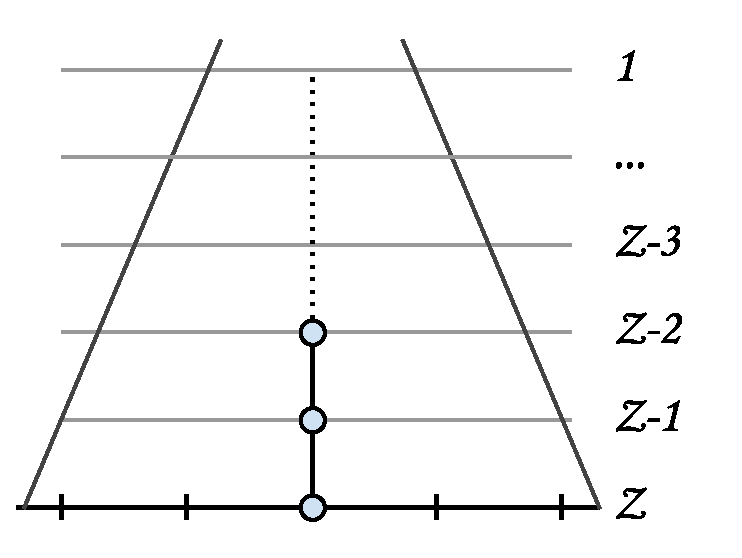
\includegraphics[scale=0.30]{figs/cvl-problem.pdf}}
  \end{center}
}

% Explain constraints
\frame
{
  \frametitle{What are constraints?}
  \begin{itemize}
  \item \textbf{Proximity constraint}: Any pair of objects must be separated by minimum distance measured in pixels on screen
  \item \textbf{Density constraint}: At most $K$ distinct objects may be visible within a tile of $256 \times 256$ pixels
  \item Users can define these constraints using special syntax (introduced next)
  \end{itemize}
  \begin{center}
  \begin{figure}
  \label{fig:contraints}
  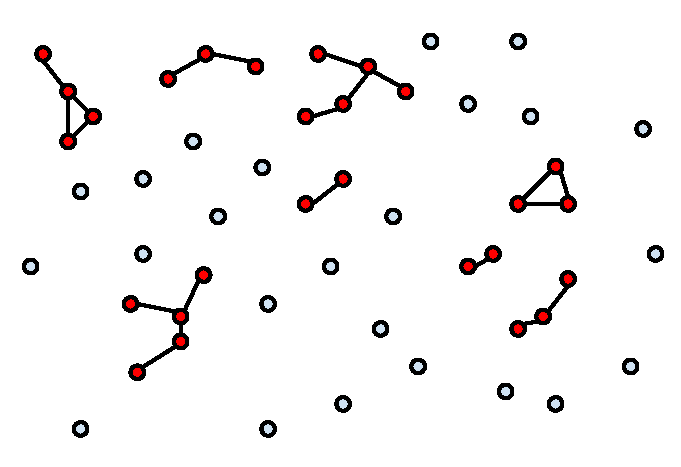
\includegraphics[scale=0.4]{figs/cvl-proximity.pdf} 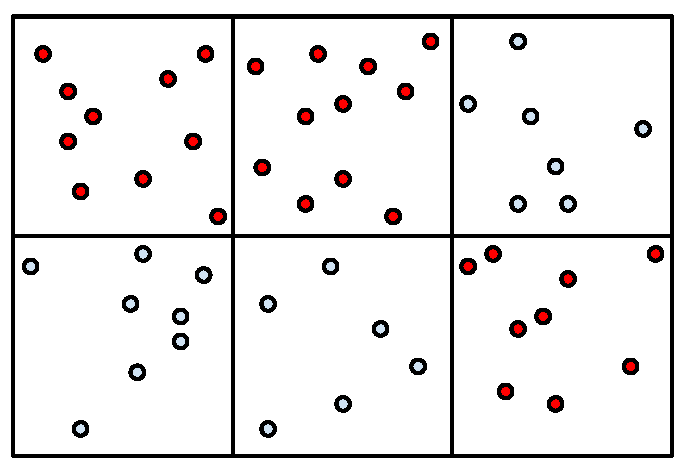
\includegraphics[scale=0.4]{figs/cvl-visibility.pdf}
  \caption{Red objects are in violation of a constraint; proximity (left) and density (right)}
  \end{figure}
  \end{center}
}

\begin{frame}[fragile]
\frametitle{CREATE CONSTRAINT statement}
\begin{lstlisting}
CREATE CONSTRAINT {Name, e.g. Proximity}
AS NOT EXISTS
  {SQL select statement}
  
RESOLVE cid IF DELETE (
  {integer expression}
)
\end{lstlisting}

\begin{itemize}
\item Programmers can use this syntax to create new constraints
\item The \texttt{AS NOT EXISTS} clause contains SQL that finds all conflicting records and groups them together by \emph{conflict ID}
\item \texttt{RESOLVE IF DELETE} clause is used to indicate how many records in a conflict group must be filtered out to resolve the conflict with the given ID
\item The term \emph{conflict} means a subset of records that violate a constraint, e.g. a pair of records that are too close vis-a-vis the proximity constraint
\end{itemize}
\end{frame}

\begin{frame}[fragile]
\frametitle{Example: Proximity constraint}
\begin{lstlisting}
CREATE CONSTRAINT Proximity
AS NOT EXISTS (
  SELECT l.id || r.id AS cid, 
    Unnest(array[l.id, r.id]) AS rid
  FROM
    {level_view} l JOIN {level_view} r
  ON
    l.id < r.id
  AND
    l.geom && ST_Expand(r.geom, 
      CVL_Resolution({z}, 256) * {parameter_1})
  AND
    ST_Distance(l.geom, r.geom) < 
      CVL_Resolution({z}, 256) * {parameter_1}
)

RESOLVE cid IF DELETE (
  1
)
\end{lstlisting}
\end{frame}

\begin{frame}[fragile]
\frametitle{Example: Proximity constraint}
\begin{center}
\fbox{The core of this constraint}
\end{center}
\begin{lstlisting}
...
(
  SELECT
    left.id || right.id AS cid, 
    Unnest(array[left.id, right.id]) AS rid
  FROM 
    {level_view} left
  JOIN 
    {level_view} right
  ON 
    ...
    ST_Distance(left.geom, right.geom) < CVL_Resolution({z}, 256) * {parameter_1}
)
...
\end{lstlisting}
\end{frame}

\begin{frame}[fragile]
\frametitle{Unbound variables}
\begin{lstlisting}
...
    {level_view}
...    
    {level_view}
...
    {z} ... {parameter_1}
...
\end{lstlisting}
\begin{itemize}
\item Variables in $\lbrace \rbrace$ are bound at runtime
\item End users, e.g. data journalists, don't need to know about variables, i.e. not used in \texttt{GENERALIZE} statement
\item Constraints are evaluated on every zoom level $\lbrace z \rbrace$
\item The $\lbrace level\_view \rbrace$ contains the currently visible records
\item A $\lbrace parameter\_n \rbrace$ is the $n$'th parameter passed to constraint in \texttt{SUBJECT TO} clause

\end{itemize}
\end{frame}

\begin{frame}[fragile,t]
  \frametitle{How to run CVL programs?}
  \begin{columns}[t]
	\begin{column}[l]{5.5cm}
		\begin{itemize}[<+->]
			\item CVL contains part SQL and part \emph{non}-SQL
  			\item SQL can be executed in spatial database 
  			\item How do we execute the \emph{non}-SQL part of CVL?
  		\end{itemize}
	\end{column}
	\begin{column}[r]{5.5cm}
\begin{lstlisting}[escapechar=@]
GENERALIZE @$\lbrace SQL \rbrace$@ 
...
WEIGH BY @$\lbrace SQL \rbrace$@
...
AS NOT EXISTS
@$\lbrace SQL \rbrace$@
RESOLVE cid IF DELETE 
@$\lbrace SQL \rbrace$@
\end{lstlisting}
	\end{column}
  \end{columns}
\end{frame}

\begin{frame}[fragile,t]
  \frametitle{How to run CVL programs?}
  \begin{columns}[t]
	\begin{column}[l]{5.5cm}
		\begin{itemize}[<+->]
			\item Compile CVL to \\$\langle$SQL + Stored Procedures$\rangle$
			\item Send to spatial database for execution!
			\item ``Send-code-to-data'' instead of ``send-data-to-code''
			\item What is the content of\\ $\langle$SQL + Stored Procedures$\rangle$?
  		\end{itemize}
	\end{column}
	\begin{column}[r]{5.5cm}
	    \begin{center}
  		%
\includegraphics[scale=0.2]{figs/light-bulb.png}
  	    \end{center}
	\end{column}
  \end{columns}
    \begin{center}
  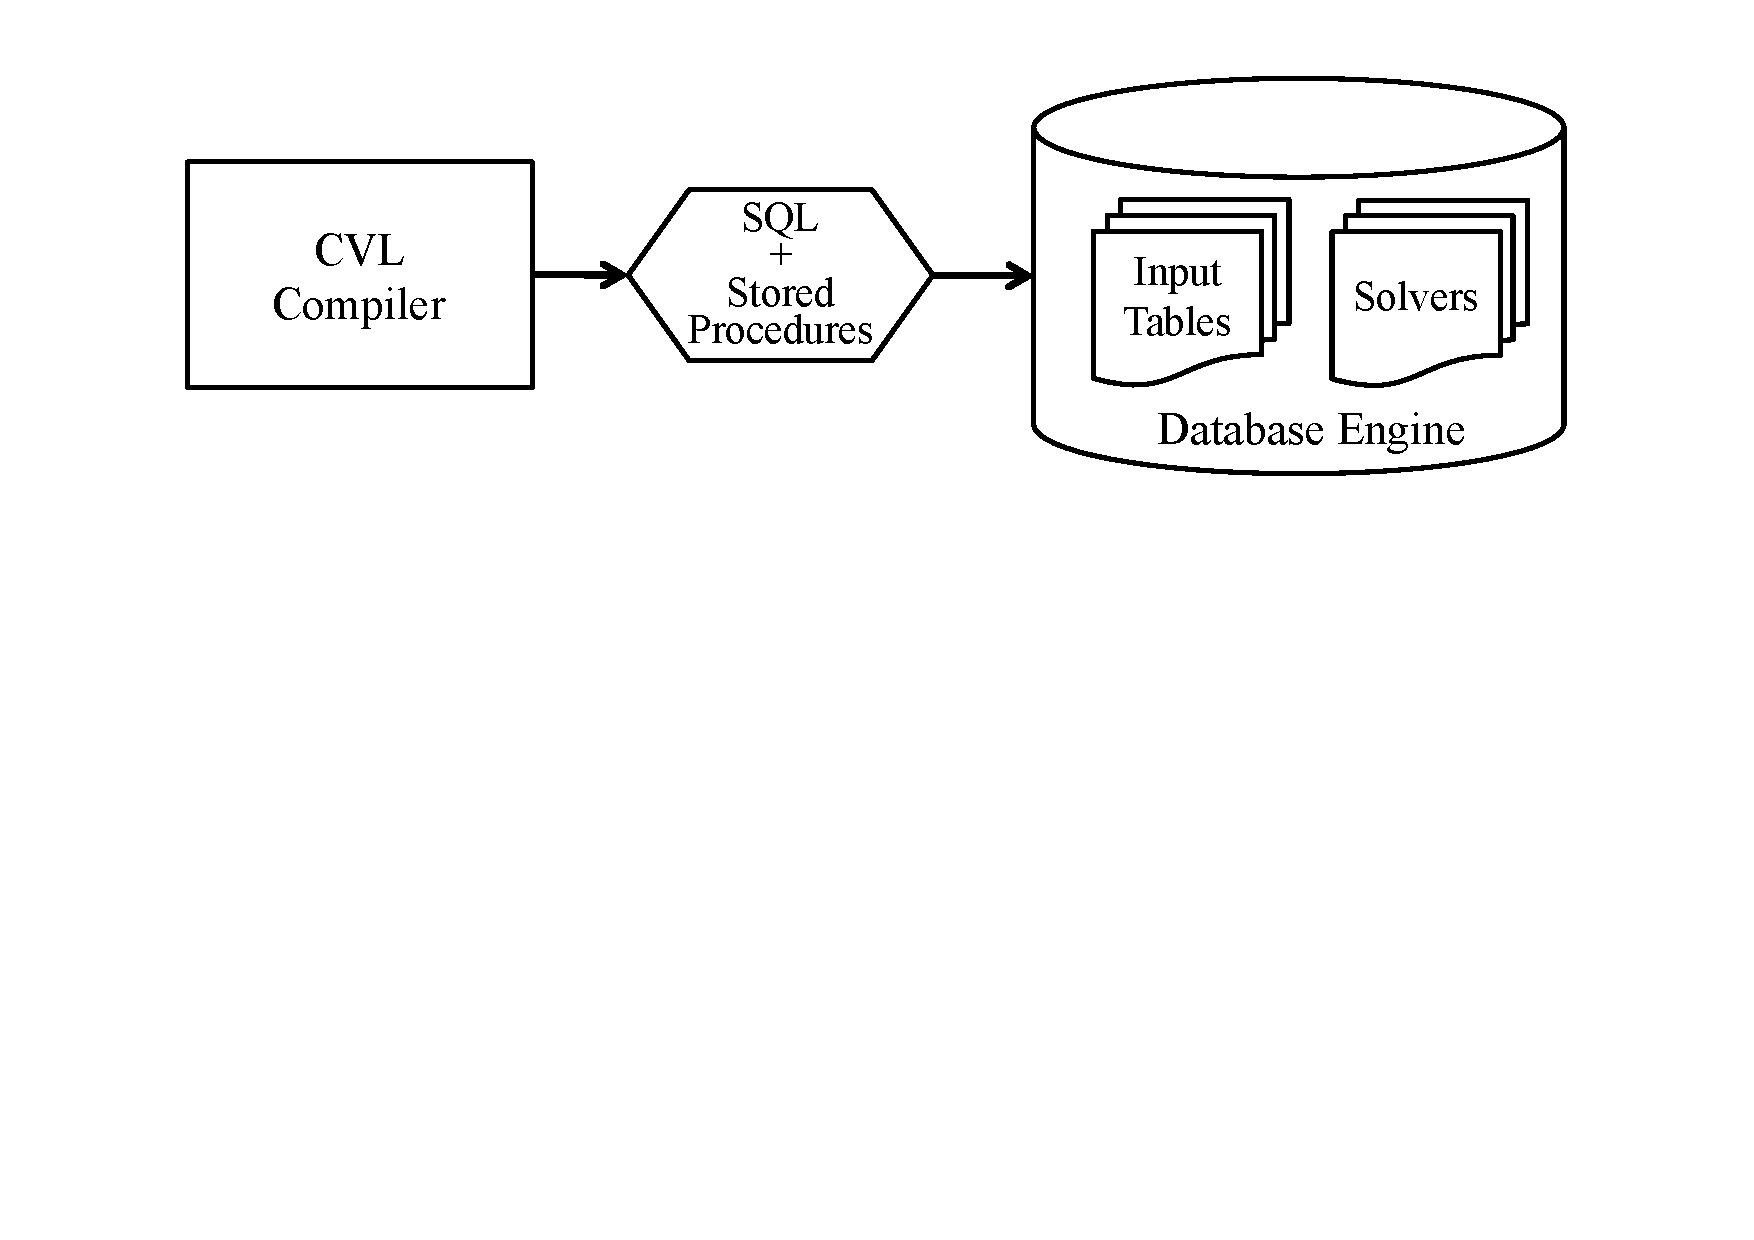
\includegraphics[scale=0.3]{figs/indatabase-execution.pdf}
  \end{center}
\end{frame}


% Last slide

\frame
{
  \frametitle{Future work}
  \begin{itemize}
  \item \textbf{Systems}: 
  \begin{enumerate}
    \item Map out design space of in-database generalization
    \item Deeper understanding of using relational algebra to solve combinatorial optimization problems
  \end{enumerate}
  \item \textbf{Language}: 
  \begin{enumerate}
  	\item Discover success and shortcomings of approach in user tests
  	\item Try other constraint and objective formulations
  	\item Other ways to resolve conflicts (e.g. aggregation)
  \end{enumerate}
  \item \textbf{Compiler}: Optimize SQL code generation
  \item \textbf{Algorithms}: Try other algorithms
  \end{itemize}
  \begin{center}
  \fbox{Thank you :-) }
  \end{center}
}


% OLD STUFF BELOW

% Overview
\frame
{
  \frametitle{Overview}
  \begin{center}
  \fbox{A view of digital web maps today :-) }
  \end{center}
  
  \begin{itemize}
  \item \textbf{OK}: Background maps are stable and of good quality (commercial and national map providers)
  \item \textbf{Challenge}: New thematic data is constantly emerging and changing (social media, sensors, ...) and needs to be visualized
  \item \textbf{Goal}: Design easy-to-use and effective \emph{programming language} for generalization that can be evaluated by a spatial database  \item \textbf{Use cases}: Data journalism, citizen information systems, crisis response, social media, ...
  \end{itemize}
}

\frame
{
  \frametitle{Map Generalization 101}
  Transforming raw spatial data\footnote{Tourism points-of-interest from OpenStreetMap}
  \begin{center}
  \fbox{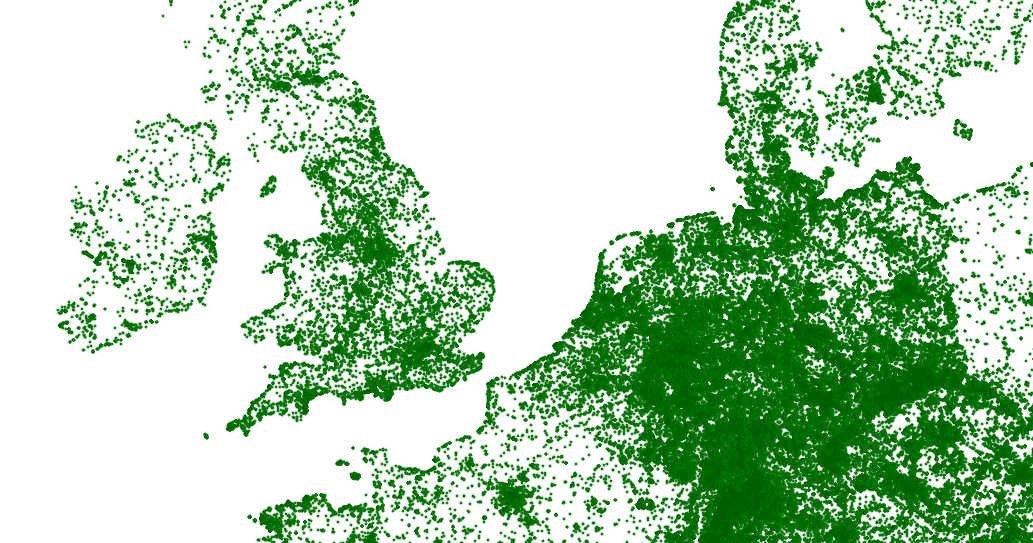
\includegraphics[scale=0.12]{figs/toomanyobjects.png}}
  \end{center}
  Into legible maps\footnote{Map created using simple random sampling of thematic point data}
  \begin{center}
  \fbox{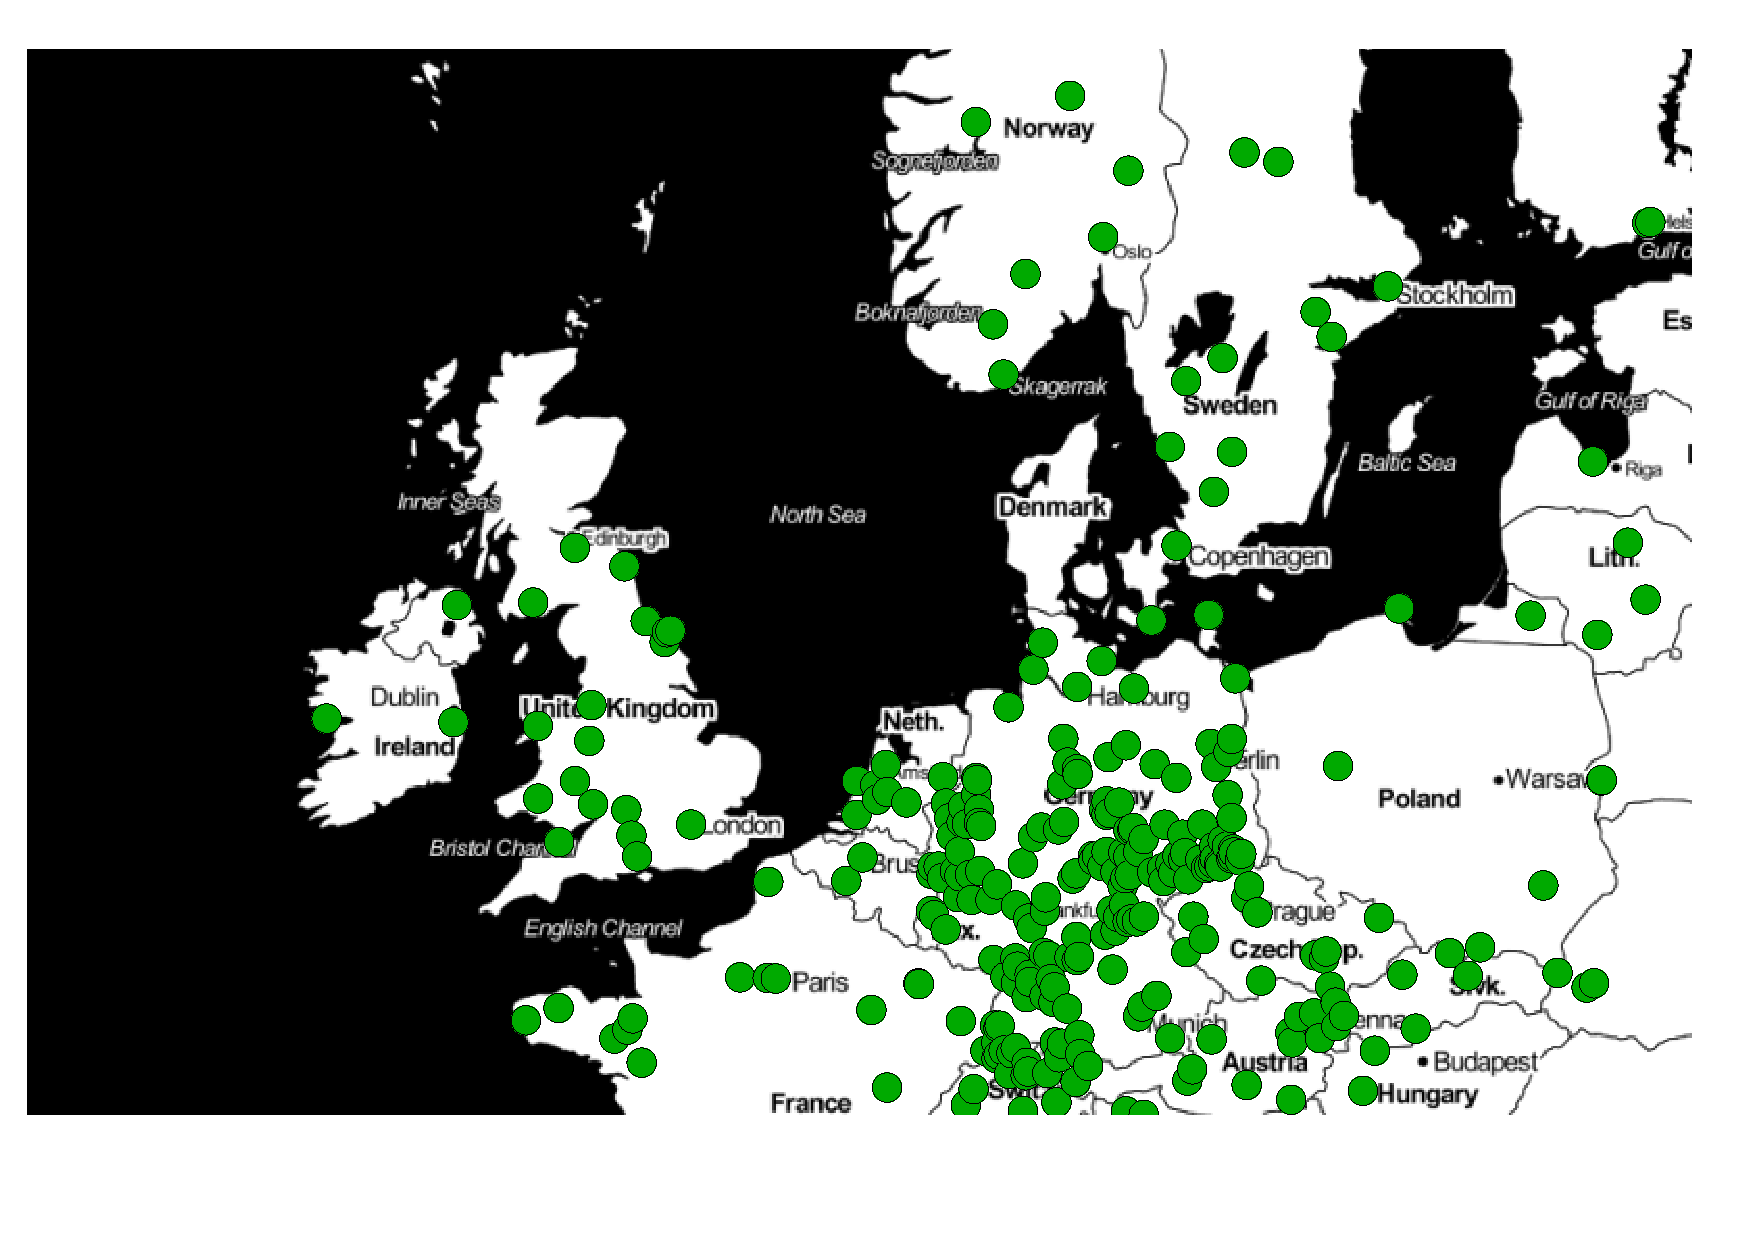
\includegraphics[scale=0.15]{figs/generalized-tourism.pdf}}
  \end{center}
}

\frame
{
  \frametitle{Questions pt 1}
  \begin{itemize}
  \item Decades of research in efficient algorithms for \emph{non}-spatial problems (Shortest Path, Travelling Salesman, Set Cover)
  \item Good algorithms exist for specific generalization problems\footnote{CS view, maybe geographers have knowledge to share here}~\cite{fusiontables,landcover}
  \item \textbf{Question}: Can we transform several related map generalization problems into a \emph{non}-spatial problem and reuse existing algorithms for this problem?
  \item \textbf{Question}: What is a good non-spatial problem to use?
  \end{itemize}
  
  \begin{center}
  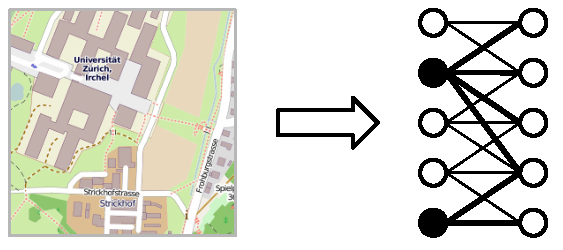
\includegraphics[scale=0.6]{figs/cvl-spatial-to-nonspatial.pdf}
  \end{center}
}

\frame
{
  \frametitle{Questions pt 2}
  \begin{itemize}
  \item A spatial database is a natural place to store spatial records
  \item However, map generalization algorithms are often implemented in specialized \emph{external software}, e.g. a Java program $\implies$ \emph{moving data in and out of database}
  \item Decades of research in database optimization
  \item Functionality includes \texttt{JOIN}, \texttt{ORDER BY}, \texttt{GROUP BY},  \texttt{CREATE INDEX} and many spatial functions: \texttt{ST\_Intersects}, \texttt{ST\_Distance}, ...
  \item \textbf{Question}: Can we formulate map generalization algorithms as a SQL transaction (with stored procedures) to be executed efficiently by a \emph{spatial database}?
  \end{itemize}
}

\begin{frame}[fragile]
  \frametitle{Questions pt 3}
  \begin{itemize}
  \item Writing complex queries in SQL is hard
  \item \textbf{Question}: Can we design a simple language that is compiled into complex SQL?
\begin{lstlisting}
GENERALIZE 
   restaurants TO restaurants2
AT 20 ZOOM LEVELS
WEIGH BY
  star_rating
SUBJECT TO 
   proximity 10
\end{lstlisting}
  \end{itemize}
\end{frame}


\frame
{
  \frametitle{Our approach}
  \begin{itemize}
  \item \textbf{Optimization}: Fit thematic generalization problem to well-known \emph{optimization problem}, i.e. \emph{set multicover problem}
  \item \textbf{Algorithms}: Survey \emph{existing algorithms} for this problem
  \item \textbf{Language}: Design an easy to use \emph{programming language} (CVL) for a class of generalization problems
  \item \textbf{Compile}: Compile CVL into a SQL transaction that generates and solves instances of the set multicover problem, and in turn solves the original generalization problem

  \end{itemize}
  \begin{center}
  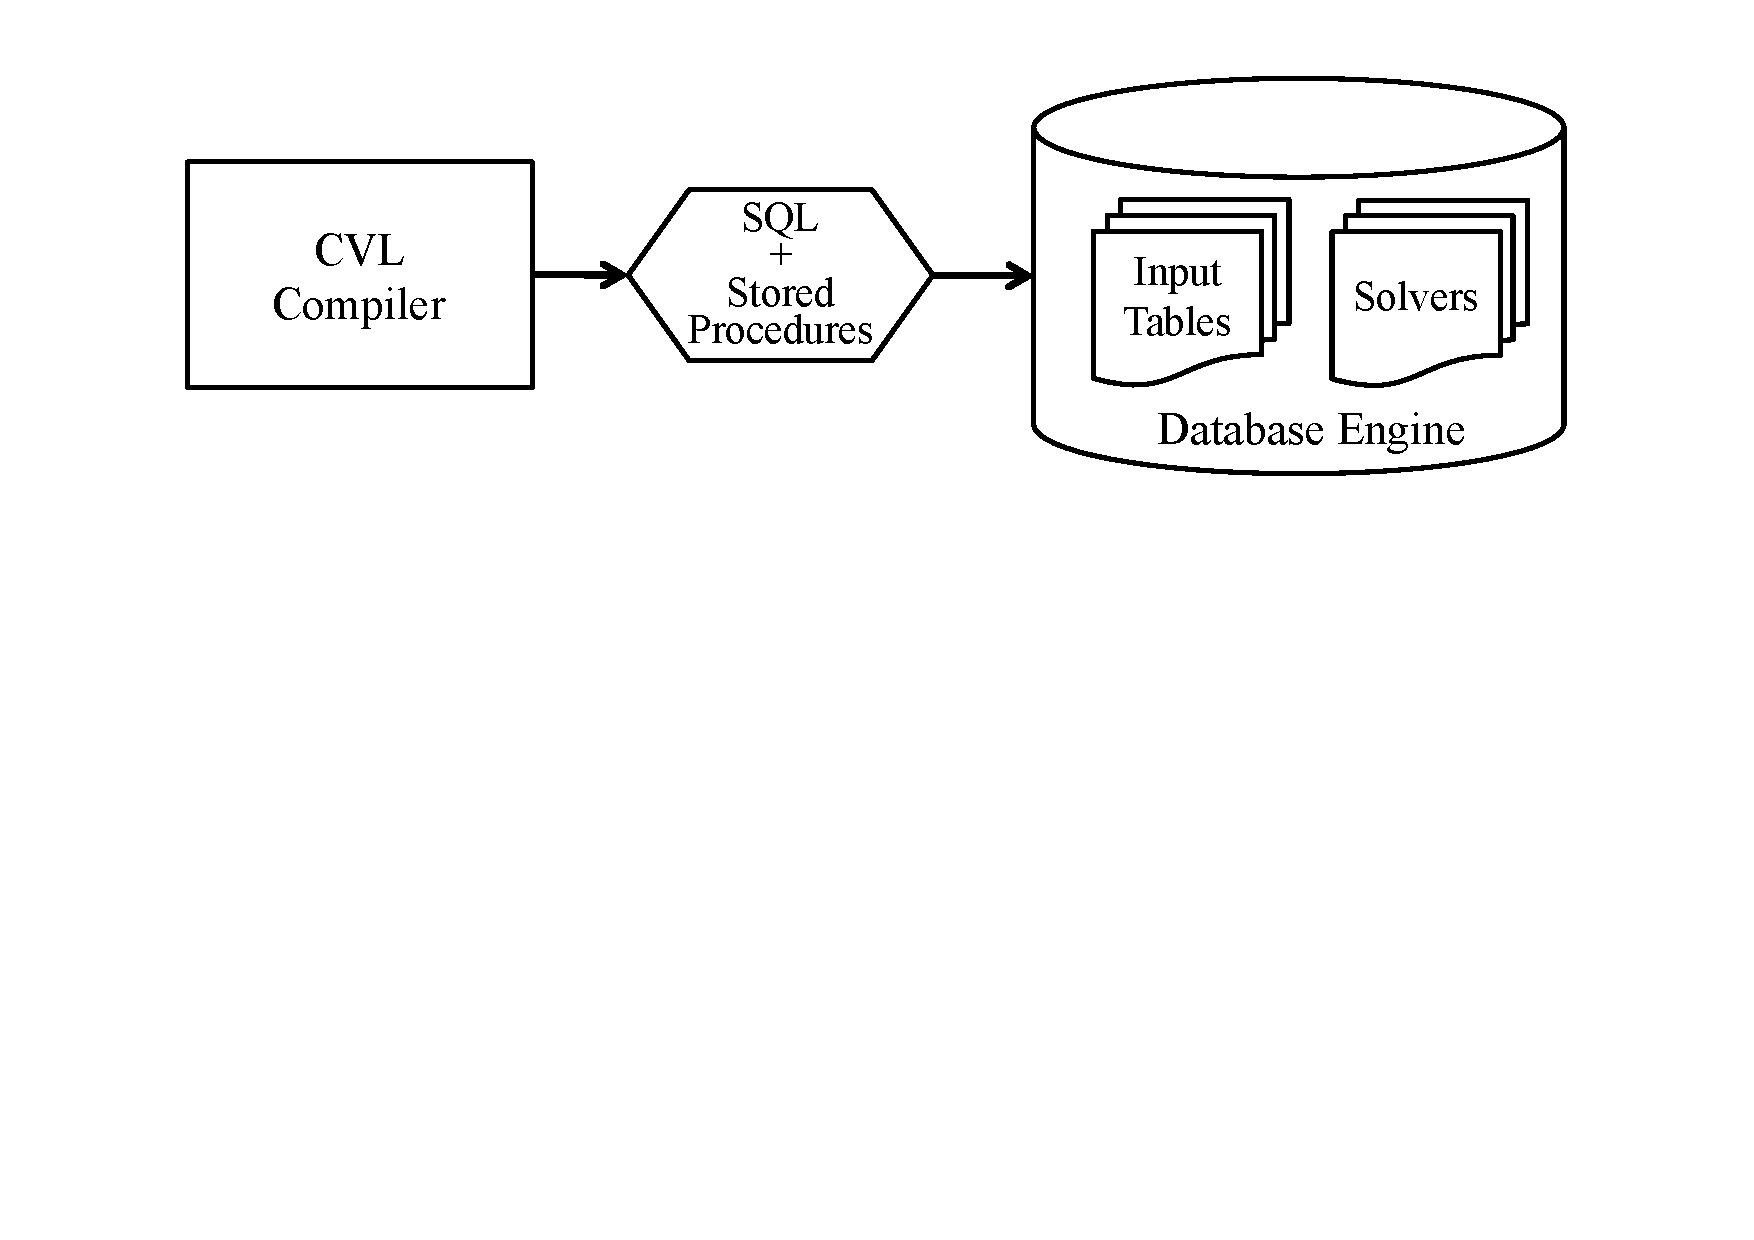
\includegraphics[scale=0.3]{figs/indatabase-execution.pdf}
  \end{center}
}

%\frame
%{
%  \frametitle{Relation to Reverse Data Management}

%  We implemented \emph{how-to} queries for spatial data:
%  \begin{itemize}
%  \item \textbf{How-to queries}~\cite{reversedatamanagement}: Given an \emph{input database}; compute an \emph{output database}, subject to set of \emph{constraints} and minimizing/maximizing an \emph{objective function}
%  \item \textbf{Spatial example}: Given an \emph{input database of spatial objects}; compute an output database that generalizes the objects to $\mathcal{Z}$ zoom-levels, subject to \emph{spatial constraints} and while \emph{minimizing loss} of objects in map (with prioritization)
%  \end{itemize}
%}

\frame
{
  \frametitle{Please note!}
  TODO: Eliminate this slide, it disrupts flow...
  
  Whenever you see the word \emph{``delete''} in this presentation, please append the words \emph{``or aggregate (future work)''} in your mind. \\
  making grammatical adjustments where appropriate.
  
  \begin{center}
  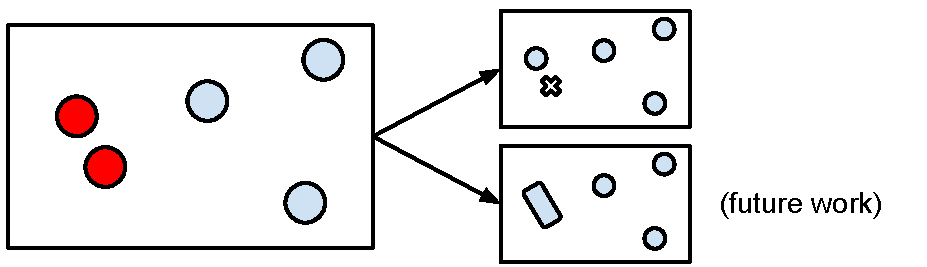
\includegraphics[scale=0.50]{figs/cvl-delete-aggregate.pdf}
  \end{center}
}


\frame
{
  \frametitle{Conflict sets}
  \begin{itemize}
  \item Model constraints (visibility, proximity, ...) using the notion of \emph{conflict sets}
  \item A conflict set is a \emph{set of objects} that cannot all appear simultaneously at a given zoom level
  \item An object can be in several conflict sets
  \item In a conflict set consisting of $k_1$ objects, where at most $k_2$ may appear in map, $\lambda = k_2 - k_1$ objects must be filtered out (deleted from current and lower zoom-levels)
  \end{itemize}
  \begin{center}
  	\fbox{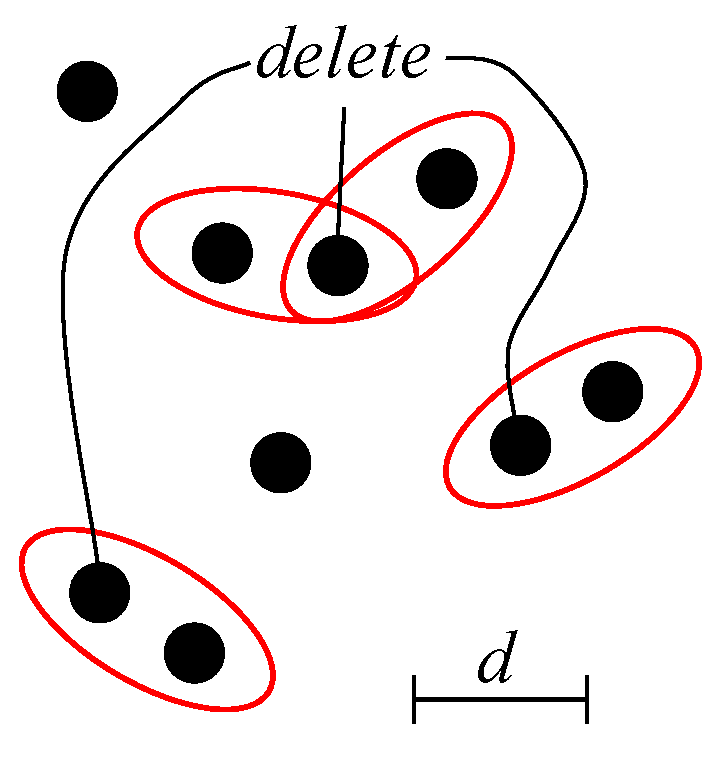
\includegraphics[scale=0.20]{figs/cvl-proximity-conflicts-2.pdf}} \fbox{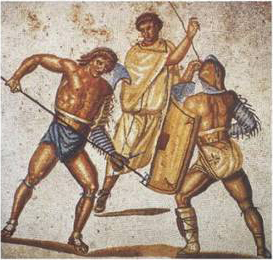
\includegraphics[scale=.38]{figs/gladiators.jpg}} \fbox{
\includegraphics[scale=.288]{figs/the-godfather-1.jpg}}
  \end{center}
}

\frame
{
  \frametitle{Single-scale filtering problem $\Leftrightarrow$ Set multicover problem}
  For each zoom-level we seek an optimal solution:
  \begin{itemize}
  \item \textbf{Set cover problem}: Given a universe $U$ of elements and a set $S$ of subsets of $U$, a \emph{cover} is a set $Q \subseteq S$ such that the union of $Q$ equals $U$.
  \item \textbf{Set multicover problem}: Each element in $e \in U$ has to be covered multiple times by $Q$.
  \item \textbf{Single-scale filtering problem}: Each conflict set $c \in C$ has to be covered multiple times times by objects that are filtered out.
  \end{itemize}
}


\begin{frame}[fragile]
\frametitle{Declarative Language for Generalization (CVL)}
\begin{itemize}
\item Language has two statements: \emph{Generalize} and \emph{Create Constraint}
\item A \emph{Generalize} statement can reference constraints defined in a \emph{Create Constraint} statement
\item Language is visually similar to SQL and uses snippets of embedded SQL
\item Designed to be compiled into SQL and executed in a database (where the data is assumed to be stored)
\end{itemize}
\end{frame}

\begin{frame}[fragile]
\frametitle{CVL: Generalize statement}
\begin{lstlisting}
GENERALIZE 
   restaurants TO restaurants_generalized
AT 20 ZOOM LEVELS
WEIGH BY
  star_rating
SUBJECT TO 
   proximity 10 AND
   visibility 64
\end{lstlisting}
\begin{itemize}
\item \texttt{restaurants} is an existing database table
\item \texttt{restaurants\_generalized} will be computed  
\item \texttt{star\_rating} used as object weight (any valid SQL expression)
\item \texttt{proximity} and \texttt{visibility} references constraints
\end{itemize}
\end{frame}


\frame
{
  \frametitle{Future work: Aggregation}
  \begin{center}
  \fbox{This is where we need your help :-)}
  \end{center}

  \begin{itemize}
  \item \textbf{User-level semantics}:
  \begin{itemize}
  \item How should user \emph{understand} aggregation, e.g. aggregation of non-geometric attributes?
  \item How should user \emph{parameterize} aggregation?
  \end{itemize}
  \item \textbf{Implementation}:
  \begin{itemize}
  \item Can we \emph{stretch} the existing model to include aggregation?
  \item Else, how does aggregation \emph{change} the problem/model?
  \item Do we need new \emph{algorithms}?
  \end{itemize}
  \end{itemize}

  \begin{center}
  \fbox{\textbf{Eiffel Tower + Louvre = ?}}
  \end{center}

}



% RELATED WORK
\frame
{
  \frametitle{Related work}

  \begin{itemize}
  \item \emph{Efficient Spatial Sampling of Large Geographical Tables}. Das Sarma, A., Lee, H., Gonzalez, H., Madhavan, J., \& Halevy, A. (2012).
  \item \emph{Reverse data management}, Meliou, A., Gatterbauer, W., \& Suciu, D. (2011).
  \item \emph{Generalization of land cover maps by mixed integer programming}. Haunert, J.-H., \& Wolff, A. (2006). 
  \item \emph{Constant information density in zoomable interfaces}. Woodruff, A., Landay, J., Stonebraker, M. (1998).
  \item And tons more of course...
  \end{itemize}
}

% Past and future work
\frame
{
  \frametitle{Past and future work}

  \begin{itemize}
  \item Past work: \emph{TileHeat}, predicting where people will look on a map tomorrow
  \item Latest work: \emph{Declarative Cartography}, the work described in these slides
  \item Future work: \emph{Real-time Declarative Cartography}, joint work with people at University of Zurich (Department of Geography)
  \item Future work: Succinct data representation of high-fidelity spatial data that is visualized on a digital map on a screen (think: pixel precision is not all that good)
  \end{itemize}
}

% Abstract view of constraints
\frame
{
  \frametitle{Constraints generate conflicts that must be resolved}
  \begin{itemize}
  \item \textbf{Constraint}: Condition (usually spatial) that must hold for subsets of records in the database on all zoom levels
  \item \textbf{Conflict}: Subset of records in database that violate a constraint, e.g. two records that are too close together
  \item \textbf{Resolving conflicts}: Make some records non-visible by setting \texttt{min\_zoom} to previous lower zoom level
  \end{itemize}
  \begin{center}
  \begin{figure}
  	\fbox{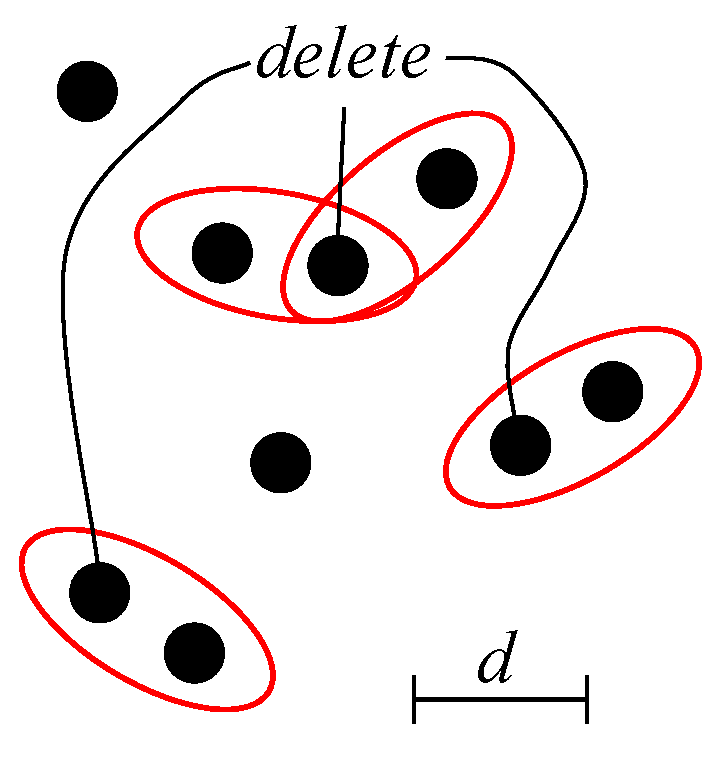
\includegraphics[scale=0.20]{figs/cvl-proximity-conflicts-2.pdf}} \fbox{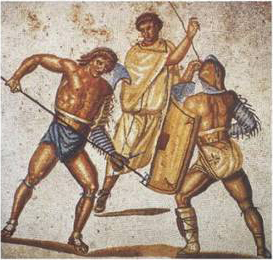
\includegraphics[scale=.38]{figs/gladiators.jpg}} \fbox{
\includegraphics[scale=.288]{figs/the-godfather-1.jpg}}
  	\caption{Resolving conflicts: Not always the survival of the most ``important'' record}
  \end{figure}
  \end{center}
}



\end{document}
